\documentclass[twoside]{book}

% Packages required by doxygen
\usepackage{fixltx2e}
\usepackage{calc}
\usepackage{doxygen}
\usepackage[export]{adjustbox} % also loads graphicx
\usepackage{graphicx}
\usepackage[utf8]{inputenc}
\usepackage{makeidx}
\usepackage{multicol}
\usepackage{multirow}
\PassOptionsToPackage{warn}{textcomp}
\usepackage{textcomp}
\usepackage[nointegrals]{wasysym}
\usepackage[table]{xcolor}

% Font selection
\usepackage[T1]{fontenc}
\usepackage[scaled=.90]{helvet}
\usepackage{courier}
\usepackage{amssymb}
\usepackage{sectsty}
\renewcommand{\familydefault}{\sfdefault}
\allsectionsfont{%
  \fontseries{bc}\selectfont%
  \color{darkgray}%
}
\renewcommand{\DoxyLabelFont}{%
  \fontseries{bc}\selectfont%
  \color{darkgray}%
}
\newcommand{\+}{\discretionary{\mbox{\scriptsize$\hookleftarrow$}}{}{}}

% Page & text layout
\usepackage{geometry}
\geometry{%
  a4paper,%
  top=2.5cm,%
  bottom=2.5cm,%
  left=2.5cm,%
  right=2.5cm%
}
\tolerance=750
\hfuzz=15pt
\hbadness=750
\setlength{\emergencystretch}{15pt}
\setlength{\parindent}{0cm}
\setlength{\parskip}{3ex plus 2ex minus 2ex}
\makeatletter
\renewcommand{\paragraph}{%
  \@startsection{paragraph}{4}{0ex}{-1.0ex}{1.0ex}{%
    \normalfont\normalsize\bfseries\SS@parafont%
  }%
}
\renewcommand{\subparagraph}{%
  \@startsection{subparagraph}{5}{0ex}{-1.0ex}{1.0ex}{%
    \normalfont\normalsize\bfseries\SS@subparafont%
  }%
}
\makeatother

% Headers & footers
\usepackage{fancyhdr}
\pagestyle{fancyplain}
\fancyhead[LE]{\fancyplain{}{\bfseries\thepage}}
\fancyhead[CE]{\fancyplain{}{}}
\fancyhead[RE]{\fancyplain{}{\bfseries\leftmark}}
\fancyhead[LO]{\fancyplain{}{\bfseries\rightmark}}
\fancyhead[CO]{\fancyplain{}{}}
\fancyhead[RO]{\fancyplain{}{\bfseries\thepage}}
\fancyfoot[LE]{\fancyplain{}{}}
\fancyfoot[CE]{\fancyplain{}{}}
\fancyfoot[RE]{\fancyplain{}{\bfseries\scriptsize Generated by Doxygen }}
\fancyfoot[LO]{\fancyplain{}{\bfseries\scriptsize Generated by Doxygen }}
\fancyfoot[CO]{\fancyplain{}{}}
\fancyfoot[RO]{\fancyplain{}{}}
\renewcommand{\footrulewidth}{0.4pt}
\renewcommand{\chaptermark}[1]{%
  \markboth{#1}{}%
}
\renewcommand{\sectionmark}[1]{%
  \markright{\thesection\ #1}%
}

% Indices & bibliography
\usepackage{natbib}
\usepackage[titles]{tocloft}
\setcounter{tocdepth}{3}
\setcounter{secnumdepth}{5}
\makeindex

% Hyperlinks (required, but should be loaded last)
\usepackage{ifpdf}
\ifpdf
  \usepackage[pdftex,pagebackref=true]{hyperref}
\else
  \usepackage[ps2pdf,pagebackref=true]{hyperref}
\fi
\hypersetup{%
  colorlinks=true,%
  linkcolor=blue,%
  citecolor=blue,%
  unicode%
}

% Custom commands
\newcommand{\clearemptydoublepage}{%
  \newpage{\pagestyle{empty}\cleardoublepage}%
}

\usepackage{caption}
\captionsetup{labelsep=space,justification=centering,font={bf},singlelinecheck=off,skip=4pt,position=top}

%===== C O N T E N T S =====

\begin{document}

% Titlepage & ToC
\hypersetup{pageanchor=false,
             bookmarksnumbered=true,
             pdfencoding=unicode
            }
\pagenumbering{roman}
\begin{titlepage}
\vspace*{7cm}
\begin{center}%
{\Large Basic implementation of D$\ast$ Lite \\[1ex]\large 1.\+0 }\\
\vspace*{1cm}
{\large Generated by Doxygen 1.8.11}\\
\end{center}
\end{titlepage}
\clearemptydoublepage
\tableofcontents
\clearemptydoublepage
\pagenumbering{arabic}
\hypersetup{pageanchor=true}

%--- Begin generated contents ---
\chapter{File Index}
\section{File List}
Here is a list of all documented files with brief descriptions\+:\begin{DoxyCompactList}
\item\contentsline{section}{app/\hyperlink{DstarLite_8cpp}{Dstar\+Lite.\+cpp} \\*Contains definitions for the planning algorithm }{\pageref{DstarLite_8cpp}}{}
\item\contentsline{section}{app/\hyperlink{Grid_8cpp}{Grid.\+cpp} \\*Contains definitions for the Grid class }{\pageref{Grid_8cpp}}{}
\item\contentsline{section}{app/\hyperlink{Node_8cpp}{Node.\+cpp} \\*Contains definitions for the Node class }{\pageref{Node_8cpp}}{}
\item\contentsline{section}{test/\hyperlink{test_8cpp}{test.\+cpp} \\*Unit tests for the path planner project }{\pageref{test_8cpp}}{}
\end{DoxyCompactList}

\chapter{File Documentation}
\hypertarget{DstarLite_8cpp}{}\section{app/\+Dstar\+Lite.cpp File Reference}
\label{DstarLite_8cpp}\index{app/\+Dstar\+Lite.\+cpp@{app/\+Dstar\+Lite.\+cpp}}


Contains definitions for the planning algorithm.  


{\ttfamily \#include \char`\"{}Dstar\+Lite.\+h\char`\"{}}\\*
{\ttfamily \#include $<$vector$>$}\\*
{\ttfamily \#include $<$algorithm$>$}\\*
{\ttfamily \#include $<$utility$>$}\\*
Include dependency graph for Dstar\+Lite.\+cpp\+:
\nopagebreak
\begin{figure}[H]
\begin{center}
\leavevmode
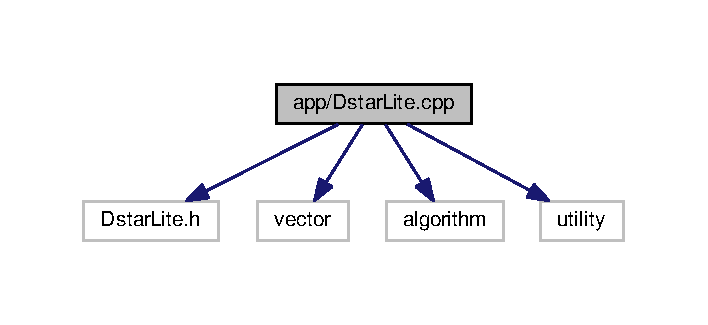
\includegraphics[width=340pt]{DstarLite_8cpp__incl}
\end{center}
\end{figure}
This graph shows which files directly or indirectly include this file\+:
\nopagebreak
\begin{figure}[H]
\begin{center}
\leavevmode
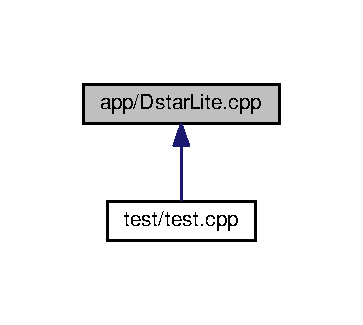
\includegraphics[width=174pt]{DstarLite_8cpp__dep__incl}
\end{center}
\end{figure}


\subsection{Detailed Description}
Contains definitions for the planning algorithm. 

This file has the definitions of the methods used in the D$\ast$ Lite algorithm

\begin{DoxyAuthor}{Author}
Pranav Dhulipala 
\end{DoxyAuthor}
\begin{DoxyDate}{Date}
10/14/2017 
\end{DoxyDate}

\hypertarget{Grid_8cpp}{}\section{app/\+Grid.cpp File Reference}
\label{Grid_8cpp}\index{app/\+Grid.\+cpp@{app/\+Grid.\+cpp}}


Contains definitions for the Grid class.  


{\ttfamily \#include \char`\"{}Grid.\+h\char`\"{}}\\*
{\ttfamily \#include $<$algorithm$>$}\\*
{\ttfamily \#include $<$vector$>$}\\*
Include dependency graph for Grid.\+cpp\+:
\nopagebreak
\begin{figure}[H]
\begin{center}
\leavevmode
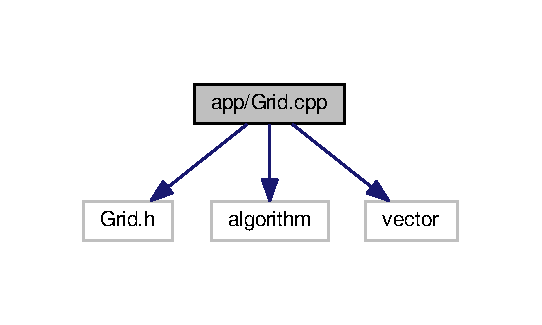
\includegraphics[width=260pt]{Grid_8cpp__incl}
\end{center}
\end{figure}
This graph shows which files directly or indirectly include this file\+:
\nopagebreak
\begin{figure}[H]
\begin{center}
\leavevmode
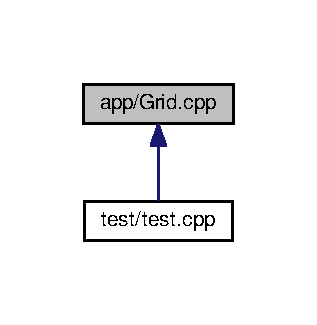
\includegraphics[width=152pt]{Grid_8cpp__dep__incl}
\end{center}
\end{figure}
\subsection*{Functions}
\begin{DoxyCompactItemize}
\item 
std\+::ostream \& \hyperlink{Grid_8cpp_a025e52017a6ddf4152f7c0fa4df92f47}{operator$<$$<$} (std\+::ostream \&out, Grid \&g)
\begin{DoxyCompactList}\small\item\em A friend of the class Grid. Overloads the ostream opertor $<$$<$ ,used to display the map. \end{DoxyCompactList}\end{DoxyCompactItemize}


\subsection{Detailed Description}
Contains definitions for the Grid class. 

This file contains the definitions of the Grid\textquotesingle{}s functionalities.

\begin{DoxyAuthor}{Author}
Pranav Dhulipala 
\end{DoxyAuthor}
\begin{DoxyDate}{Date}
10/14/2017 
\end{DoxyDate}


\subsection{Function Documentation}
\index{Grid.\+cpp@{Grid.\+cpp}!operator$<$$<$@{operator$<$$<$}}
\index{operator$<$$<$@{operator$<$$<$}!Grid.\+cpp@{Grid.\+cpp}}
\subsubsection[{\texorpdfstring{operator$<$$<$(std\+::ostream \&out, Grid \&g)}{operator<<(std::ostream &out, Grid &g)}}]{\setlength{\rightskip}{0pt plus 5cm}std\+::ostream\& operator$<$$<$ (
\begin{DoxyParamCaption}
\item[{std\+::ostream \&}]{out, }
\item[{Grid \&}]{g}
\end{DoxyParamCaption}
)}\hypertarget{Grid_8cpp_a025e52017a6ddf4152f7c0fa4df92f47}{}\label{Grid_8cpp_a025e52017a6ddf4152f7c0fa4df92f47}


A friend of the class Grid. Overloads the ostream opertor $<$$<$ ,used to display the map. 


\begin{DoxyParams}{Parameters}
{\em out} & is a reference of an ostream object \\
\hline
{\em g} & is a reference of a Grid object \\
\hline
\end{DoxyParams}
\begin{DoxyReturn}{Returns}
overloads the $<$$<$ operator 
\end{DoxyReturn}

\hypertarget{Node_8cpp}{}\section{app/\+Node.cpp File Reference}
\label{Node_8cpp}\index{app/\+Node.\+cpp@{app/\+Node.\+cpp}}


Contains definitions for the Node class.  


{\ttfamily \#include \char`\"{}Node.\+h\char`\"{}}\\*
{\ttfamily \#include $<$utility$>$}\\*
Include dependency graph for Node.\+cpp\+:
\nopagebreak
\begin{figure}[H]
\begin{center}
\leavevmode
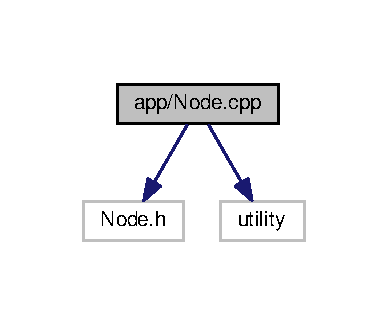
\includegraphics[width=186pt]{Node_8cpp__incl}
\end{center}
\end{figure}
This graph shows which files directly or indirectly include this file\+:
\nopagebreak
\begin{figure}[H]
\begin{center}
\leavevmode
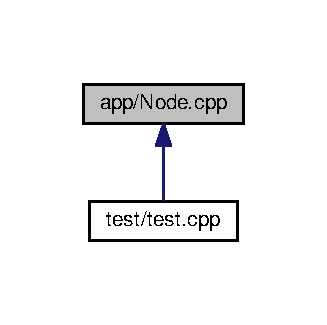
\includegraphics[width=157pt]{Node_8cpp__dep__incl}
\end{center}
\end{figure}
\subsection*{Functions}
\begin{DoxyCompactItemize}
\item 
const Node \hyperlink{Node_8cpp_a0aaf9b7cb137790dd835d7b12b335948}{operator+} (const Node \&l, const Node \&r)
\begin{DoxyCompactList}\small\item\em A friend to the class Node. Overloads the operator +, used to add two const Node obejcts. \end{DoxyCompactList}\item 
bool \hyperlink{Node_8cpp_a78329d67ea8594d125bd6ab292773f47}{operator==} (const Node \&l, const Node \&r)
\begin{DoxyCompactList}\small\item\em A friend to the class Node.\+Overloads the operator ==, used to check if the two const Node elements are the same. \end{DoxyCompactList}\item 
bool \hyperlink{Node_8cpp_a0659b04d4c436b42ac754c33eb887960}{operator!=} (const Node \&l, const Node \&r)
\begin{DoxyCompactList}\small\item\em A friend to the class Node.\+Overloads the operator !=, used to check if the two const Node elements are different. \end{DoxyCompactList}\end{DoxyCompactItemize}


\subsection{Detailed Description}
Contains definitions for the Node class. 

This file has the definitions of the methods used in the Node header

\begin{DoxyAuthor}{Author}
Pranav Dhulipala 
\end{DoxyAuthor}
\begin{DoxyDate}{Date}
10/14/2017 
\end{DoxyDate}


\subsection{Function Documentation}
\index{Node.\+cpp@{Node.\+cpp}!operator"!=@{operator"!=}}
\index{operator"!=@{operator"!=}!Node.\+cpp@{Node.\+cpp}}
\subsubsection[{\texorpdfstring{operator"!=(const Node \&l, const Node \&r)}{operator!=(const Node &l, const Node &r)}}]{\setlength{\rightskip}{0pt plus 5cm}bool operator!= (
\begin{DoxyParamCaption}
\item[{const Node \&}]{l, }
\item[{const Node \&}]{r}
\end{DoxyParamCaption}
)}\hypertarget{Node_8cpp_a0659b04d4c436b42ac754c33eb887960}{}\label{Node_8cpp_a0659b04d4c436b42ac754c33eb887960}


A friend to the class Node.\+Overloads the operator !=, used to check if the two const Node elements are different. 


\begin{DoxyParams}{Parameters}
{\em r} & a reference of the const Node class object \\
\hline
{\em l} & a reference of the const Node class object \\
\hline
\end{DoxyParams}
\begin{DoxyReturn}{Returns}
a bool value, true if the elements are not equal false if equal 
\end{DoxyReturn}
\index{Node.\+cpp@{Node.\+cpp}!operator+@{operator+}}
\index{operator+@{operator+}!Node.\+cpp@{Node.\+cpp}}
\subsubsection[{\texorpdfstring{operator+(const Node \&l, const Node \&r)}{operator+(const Node &l, const Node &r)}}]{\setlength{\rightskip}{0pt plus 5cm}const Node operator+ (
\begin{DoxyParamCaption}
\item[{const Node \&}]{l, }
\item[{const Node \&}]{r}
\end{DoxyParamCaption}
)}\hypertarget{Node_8cpp_a0aaf9b7cb137790dd835d7b12b335948}{}\label{Node_8cpp_a0aaf9b7cb137790dd835d7b12b335948}


A friend to the class Node. Overloads the operator +, used to add two const Node obejcts. 


\begin{DoxyParams}{Parameters}
{\em r} & a reference of the Node class object \\
\hline
{\em l} & a reference of the Node class object \\
\hline
\end{DoxyParams}
\begin{DoxyReturn}{Returns}
a const Node created by adding the \+\_\+x and \+\_\+y values of the parameters 
\end{DoxyReturn}
\index{Node.\+cpp@{Node.\+cpp}!operator==@{operator==}}
\index{operator==@{operator==}!Node.\+cpp@{Node.\+cpp}}
\subsubsection[{\texorpdfstring{operator==(const Node \&l, const Node \&r)}{operator==(const Node &l, const Node &r)}}]{\setlength{\rightskip}{0pt plus 5cm}bool operator== (
\begin{DoxyParamCaption}
\item[{const Node \&}]{l, }
\item[{const Node \&}]{r}
\end{DoxyParamCaption}
)}\hypertarget{Node_8cpp_a78329d67ea8594d125bd6ab292773f47}{}\label{Node_8cpp_a78329d67ea8594d125bd6ab292773f47}


A friend to the class Node.\+Overloads the operator ==, used to check if the two const Node elements are the same. 


\begin{DoxyParams}{Parameters}
{\em r} & a reference of the const Node class object \\
\hline
{\em l} & a reference of the const Node class object \\
\hline
\end{DoxyParams}
\begin{DoxyReturn}{Returns}
a bool value, true if the elements are equal false if different 
\end{DoxyReturn}

\hypertarget{test_8cpp}{}\section{test/test.cpp File Reference}
\label{test_8cpp}\index{test/test.\+cpp@{test/test.\+cpp}}


Unit tests for the path planner project.  


{\ttfamily \#include $<$gtest/gtest.\+h$>$}\\*
{\ttfamily \#include $<$utility$>$}\\*
{\ttfamily \#include $<$iostream$>$}\\*
{\ttfamily \#include $<$vector$>$}\\*
{\ttfamily \#include \char`\"{}../include/\+Node.\+h\char`\"{}}\\*
{\ttfamily \#include \char`\"{}../app/\+Node.\+cpp\char`\"{}}\\*
{\ttfamily \#include \char`\"{}../include/\+Grid.\+h\char`\"{}}\\*
{\ttfamily \#include \char`\"{}../app/\+Grid.\+cpp\char`\"{}}\\*
{\ttfamily \#include \char`\"{}../include/\+Dstar\+Lite.\+h\char`\"{}}\\*
{\ttfamily \#include \char`\"{}../app/\+Dstar\+Lite.\+cpp\char`\"{}}\\*
Include dependency graph for test.\+cpp\+:
\nopagebreak
\begin{figure}[H]
\begin{center}
\leavevmode
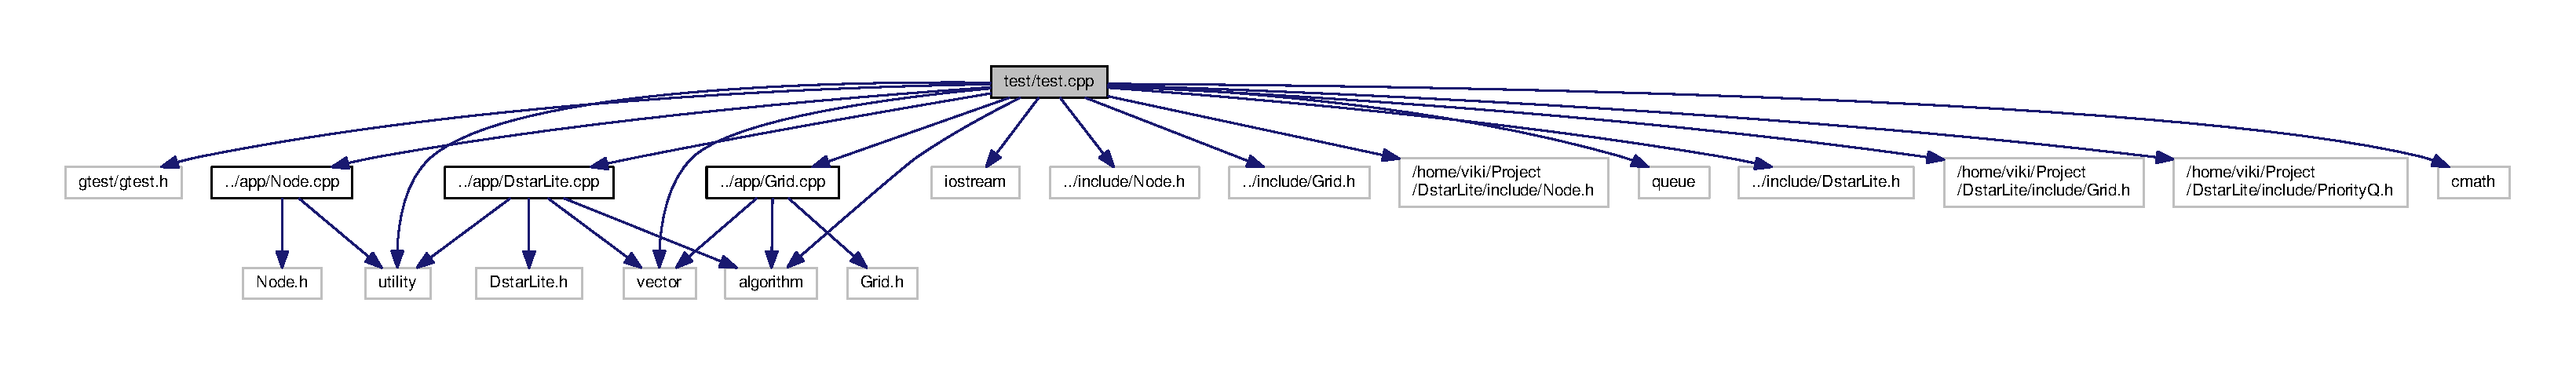
\includegraphics[width=350pt]{test_8cpp__incl}
\end{center}
\end{figure}
\subsection*{Functions}
\begin{DoxyCompactItemize}
\item 
\hyperlink{test_8cpp_a61e6db502ddaabf8db6891ce2cb7aea2}{T\+E\+ST} (Node\+Test, Not\+Negative)\hypertarget{test_8cpp_a61e6db502ddaabf8db6891ce2cb7aea2}{}\label{test_8cpp_a61e6db502ddaabf8db6891ce2cb7aea2}

\begin{DoxyCompactList}\small\item\em Checks if the coordinates of Node are not negative. \end{DoxyCompactList}\item 
\hyperlink{test_8cpp_a25205d2841e73a0b6e1a53d91b4fb05c}{T\+E\+ST} (Node\+Key\+Test, Not\+Negative)\hypertarget{test_8cpp_a25205d2841e73a0b6e1a53d91b4fb05c}{}\label{test_8cpp_a25205d2841e73a0b6e1a53d91b4fb05c}

\begin{DoxyCompactList}\small\item\em Checks if the key values of the Node are not negative. \end{DoxyCompactList}\item 
\hyperlink{test_8cpp_afdbe9030904029801d6e6d42b9339306}{T\+E\+ST} (Node\+Equal\+Test, Equal)\hypertarget{test_8cpp_afdbe9030904029801d6e6d42b9339306}{}\label{test_8cpp_afdbe9030904029801d6e6d42b9339306}

\begin{DoxyCompactList}\small\item\em Checks if the operator overloading of +,== work. \end{DoxyCompactList}\item 
\hyperlink{test_8cpp_ac8207678e016b3e6fd447ff3c65bcc5f}{T\+E\+ST} (Node\+Default\+Test, True)\hypertarget{test_8cpp_ac8207678e016b3e6fd447ff3c65bcc5f}{}\label{test_8cpp_ac8207678e016b3e6fd447ff3c65bcc5f}

\begin{DoxyCompactList}\small\item\em checks if the node default constructor initializes \+\_\+x,\+\_\+y as 0 \end{DoxyCompactList}\item 
\hyperlink{test_8cpp_a105d0c8ac5ef006cf33680e2bef1cf21}{T\+E\+ST} (Node\+Constructor\+Test, Equal)\hypertarget{test_8cpp_a105d0c8ac5ef006cf33680e2bef1cf21}{}\label{test_8cpp_a105d0c8ac5ef006cf33680e2bef1cf21}

\begin{DoxyCompactList}\small\item\em checks the constructor taking Node objects functionality \end{DoxyCompactList}\item 
\hyperlink{test_8cpp_a22c3c9be661011fa0cc5f05450ecf984}{T\+E\+ST} (Node\+Key\+Test, True)\hypertarget{test_8cpp_a22c3c9be661011fa0cc5f05450ecf984}{}\label{test_8cpp_a22c3c9be661011fa0cc5f05450ecf984}

\begin{DoxyCompactList}\small\item\em checks the setkey and getkey methods \end{DoxyCompactList}\item 
\hyperlink{test_8cpp_acfa2ebcb387d7f48852b468e787d29ac}{T\+E\+ST} (Node\+Key\+Compare, Less\+Than)\hypertarget{test_8cpp_acfa2ebcb387d7f48852b468e787d29ac}{}\label{test_8cpp_acfa2ebcb387d7f48852b468e787d29ac}

\begin{DoxyCompactList}\small\item\em checks if the key value is less than second key value \end{DoxyCompactList}\item 
\hyperlink{test_8cpp_a3da76b28dc986f7a90c220d1911e0cb2}{T\+E\+ST} (Node\+Key\+Compare, True)\hypertarget{test_8cpp_a3da76b28dc986f7a90c220d1911e0cb2}{}\label{test_8cpp_a3da76b28dc986f7a90c220d1911e0cb2}

\begin{DoxyCompactList}\small\item\em checks if the key value is less than second key value \end{DoxyCompactList}\item 
\hyperlink{test_8cpp_aee978daed33a6f38a05d3a5bc6bf9bd2}{T\+E\+ST} (Node\+Key\+Compare, False)\hypertarget{test_8cpp_aee978daed33a6f38a05d3a5bc6bf9bd2}{}\label{test_8cpp_aee978daed33a6f38a05d3a5bc6bf9bd2}

\begin{DoxyCompactList}\small\item\em checks if the key value is less than second key value \end{DoxyCompactList}\item 
\hyperlink{test_8cpp_a066b340f096988302025083003504d8f}{T\+E\+ST} (Node\+Not\+Equal\+Test, Not\+Equal)\hypertarget{test_8cpp_a066b340f096988302025083003504d8f}{}\label{test_8cpp_a066b340f096988302025083003504d8f}

\begin{DoxyCompactList}\small\item\em Checks if the operator overloading of +,!= work. \end{DoxyCompactList}\item 
\hyperlink{test_8cpp_ae8b18cc749c1fcca4ed0466c0b8692b7}{T\+E\+ST} (Obstacle\+Check, In\+Obstacle)\hypertarget{test_8cpp_ae8b18cc749c1fcca4ed0466c0b8692b7}{}\label{test_8cpp_ae8b18cc749c1fcca4ed0466c0b8692b7}

\begin{DoxyCompactList}\small\item\em Checks if the Node is in the obstacle. Checks the obstacle method. \end{DoxyCompactList}\item 
\hyperlink{test_8cpp_a980e4b785b3d484297525505aaded02a}{T\+E\+ST} (Node\+Valid, Valid)\hypertarget{test_8cpp_a980e4b785b3d484297525505aaded02a}{}\label{test_8cpp_a980e4b785b3d484297525505aaded02a}

\begin{DoxyCompactList}\small\item\em Checks if the Node is valid. Checks the is\+Valid function. \end{DoxyCompactList}\item 
\hyperlink{test_8cpp_add2f86f4836de4dd758076ec0e260944}{T\+E\+ST} (Heuristic\+Value, Equal)\hypertarget{test_8cpp_add2f86f4836de4dd758076ec0e260944}{}\label{test_8cpp_add2f86f4836de4dd758076ec0e260944}

\begin{DoxyCompactList}\small\item\em Checks if the value returned by the heuristic function is equal to the known value. Checks the heuristic function. \end{DoxyCompactList}\item 
\hyperlink{test_8cpp_a652ee2762f292c526bf649055255d5cf}{T\+E\+ST} (Priority\+Q\+Min\+Test, Min\+Element\+Equal)\hypertarget{test_8cpp_a652ee2762f292c526bf649055255d5cf}{}\label{test_8cpp_a652ee2762f292c526bf649055255d5cf}

\begin{DoxyCompactList}\small\item\em Checks if the priority queue sorts the Nodes based on the key values, is equal to the known Node with lowest key values. Checks if the comparator of PriorityQ works. \end{DoxyCompactList}\item 
\hyperlink{test_8cpp_a818006fe7bace0e1de4bc0fad9a88e9e}{T\+E\+ST} (Priority\+Q\+Find\+Element\+Test, Element\+Not\+Found)\hypertarget{test_8cpp_a818006fe7bace0e1de4bc0fad9a88e9e}{}\label{test_8cpp_a818006fe7bace0e1de4bc0fad9a88e9e}

\begin{DoxyCompactList}\small\item\em Checks if the priority queue contains the removed Node. Checks the remove and find methods of the PriorityQ. \end{DoxyCompactList}\item 
\hyperlink{test_8cpp_a6b10294cece388c2d7c98aec0948846f}{T\+E\+ST} (Comparator\+Test, False)\hypertarget{test_8cpp_a6b10294cece388c2d7c98aec0948846f}{}\label{test_8cpp_a6b10294cece388c2d7c98aec0948846f}

\begin{DoxyCompactList}\small\item\em checks the struct compare \end{DoxyCompactList}\item 
\hyperlink{test_8cpp_ae6f1e8a4873ad835a1900cb8c147d9a0}{T\+E\+ST} (Comparator\+Test, True)\hypertarget{test_8cpp_ae6f1e8a4873ad835a1900cb8c147d9a0}{}\label{test_8cpp_ae6f1e8a4873ad835a1900cb8c147d9a0}

\begin{DoxyCompactList}\small\item\em checks the struct compare \end{DoxyCompactList}\item 
\hyperlink{test_8cpp_a8de07acc1843389eda83f4dfdc88e067}{T\+E\+ST} (Comparator\+Test, Also\+False)\hypertarget{test_8cpp_a8de07acc1843389eda83f4dfdc88e067}{}\label{test_8cpp_a8de07acc1843389eda83f4dfdc88e067}

\begin{DoxyCompactList}\small\item\em checks the struct compare \end{DoxyCompactList}\item 
\hyperlink{test_8cpp_aced0c23f6c626326b4ee1d63c3e66466}{T\+E\+ST} (Priority\+Q\+Remove\+Element\+Test, False)\hypertarget{test_8cpp_aced0c23f6c626326b4ee1d63c3e66466}{}\label{test_8cpp_aced0c23f6c626326b4ee1d63c3e66466}

\begin{DoxyCompactList}\small\item\em Checks if the priority queue contains the removed Node. \end{DoxyCompactList}\item 
\hyperlink{test_8cpp_a0b93424211b96aa26e401a08e01f657c}{T\+E\+ST} (Ostream\+Test, True)\hypertarget{test_8cpp_a0b93424211b96aa26e401a08e01f657c}{}\label{test_8cpp_a0b93424211b96aa26e401a08e01f657c}

\begin{DoxyCompactList}\small\item\em checks operator $<$$<$ overload \end{DoxyCompactList}\item 
\hyperlink{test_8cpp_a88a74ac95a473843e47b4e61034d61b4}{T\+E\+ST} (Initialize\+Test, Equal)\hypertarget{test_8cpp_a88a74ac95a473843e47b4e61034d61b4}{}\label{test_8cpp_a88a74ac95a473843e47b4e61034d61b4}

\begin{DoxyCompactList}\small\item\em checks if initialize method works by checking if the goal rhs is set to 0 \end{DoxyCompactList}\item 
\hyperlink{test_8cpp_a49c310aaaf73a052c8892226634610c1}{T\+E\+ST} (Neighbour\+Test, Equal)\hypertarget{test_8cpp_a49c310aaaf73a052c8892226634610c1}{}\label{test_8cpp_a49c310aaaf73a052c8892226634610c1}

\begin{DoxyCompactList}\small\item\em checks the functionality of the neighbour method by checking if all the 8 neighbours are returned \end{DoxyCompactList}\item 
\hyperlink{test_8cpp_af4b89bd05ee655d8bf93b433fd228a91}{T\+E\+ST} (Calculate\+Key\+Test, Less\+Than)\hypertarget{test_8cpp_af4b89bd05ee655d8bf93b433fd228a91}{}\label{test_8cpp_af4b89bd05ee655d8bf93b433fd228a91}

\begin{DoxyCompactList}\small\item\em checks the functionality of calculate key by comparing the key values \end{DoxyCompactList}\item 
\hyperlink{test_8cpp_a88aee11a8927221451858be664e34ca3}{T\+E\+ST} (Scan\+Test, Not\+Equal)\hypertarget{test_8cpp_a88aee11a8927221451858be664e34ca3}{}\label{test_8cpp_a88aee11a8927221451858be664e34ca3}

\begin{DoxyCompactList}\small\item\em checks the functionality of Scan methods by checking the vector size returned is greater than 8 the node\textquotesingle{}s actual neighbours \end{DoxyCompactList}\item 
\hyperlink{test_8cpp_a7ffa8e347520830827c7878a33b9e011}{T\+E\+ST} (Compute\+Path\+Test, Notequal)\hypertarget{test_8cpp_a7ffa8e347520830827c7878a33b9e011}{}\label{test_8cpp_a7ffa8e347520830827c7878a33b9e011}

\begin{DoxyCompactList}\small\item\em checks if the compute path and update\+Vertex methods work by checking the initial rhs value of the last node and its new value after running the functions \end{DoxyCompactList}\end{DoxyCompactItemize}


\subsection{Detailed Description}
Unit tests for the path planner project. 

This file contains implementation of unit tests for this project

\begin{DoxyAuthor}{Author}
Pranav Dhulipala 
\end{DoxyAuthor}
\begin{DoxyVersion}{Version}
1.\+0 
\end{DoxyVersion}

%--- End generated contents ---

% Index
\backmatter
\newpage
\phantomsection
\clearemptydoublepage
\addcontentsline{toc}{chapter}{Index}
\printindex

\end{document}
